% generated by plots/fig8_reasoning.py --- do not edit the numbers by hand
% figure* --- the chapter is two-column and this does not fit one
\begin{figure*}[tp]
\centering
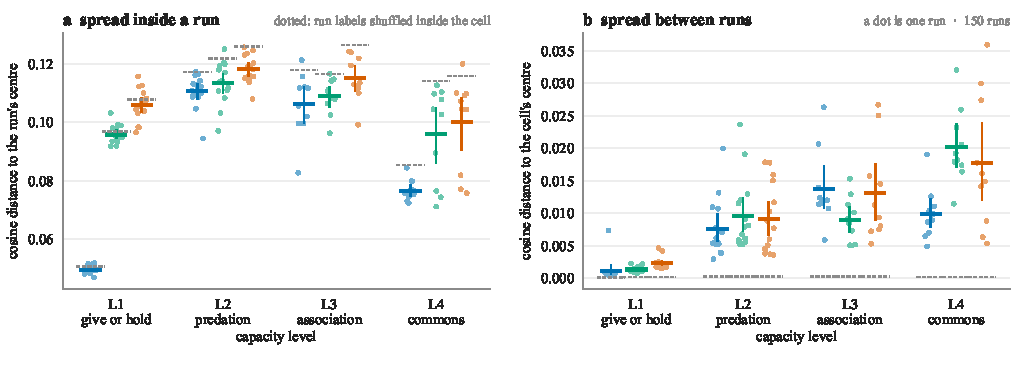
\includegraphics[width=\linewidth]{figures/fig8_reasoning/dispersion.pdf}\\[2pt]
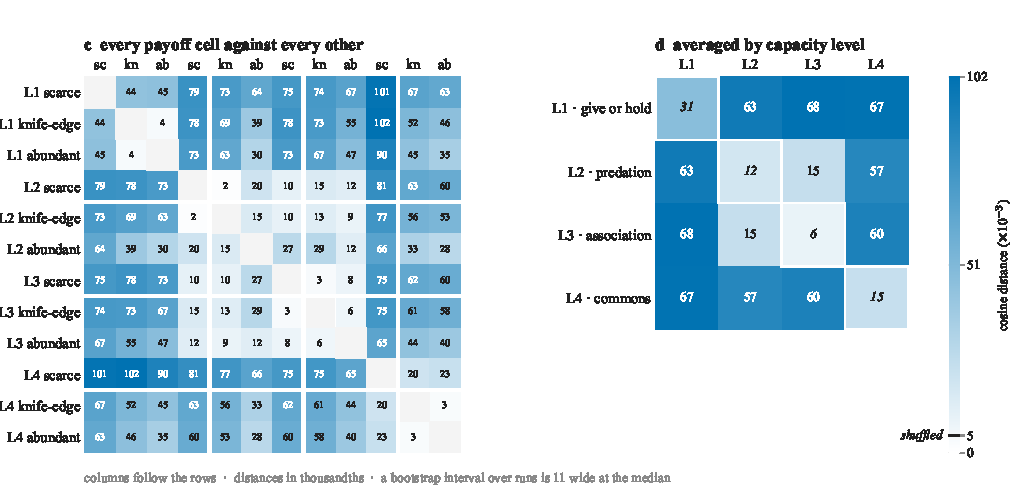
\includegraphics[width=\linewidth]{figures/fig8_reasoning/matrix.pdf}\\[2pt]
\caption[Reasoning traces in embedding space]{%
\textbf{Reasoning traces in embedding space.} How alike the reasoning of the twelve payoff cells is, read off the text the agents wrote while deciding. The view is exploratory: nothing in it is a test and no p-value is computed anywhere. \textbf{(a, b)} The spread of a payoff cell split in two, both in cosine distance and on one scale: how far a run's traces sit from that run's own centre, and how far each run's centre sits from the centre of its cell. A dot is one of the 150 runs, the bar is the cell mean with a 95\% interval over runs, and the dotted rule is the same quantity with the run labels shuffled inside the cell. The distance inside a run is the larger by a factor of 11 (0.100 against 0.009) and comes within 7 per cent of its shuffled rule, so which run a trace came from says little about how it is worded. The distance between runs is instead 8 to 99 times its shuffled rule in every cell, and rises with every step of the ladder, from 0.002 at L1 to 0.016 at L4. The narrowest cell is L1 scarce at 0.050, the widest L2 abundant at 0.118. \textbf{(c, d)} Cosine distance between the centres of the twelve cells, in thousandths, with the shuffled reference marked on the bar; (d) averages the same numbers by capacity level, its diagonal being the mean distance among a level's own three payoff cells. The capacity level accounts for most of what separates the cells: L1 and L3 sit 68 apart while L2 and L3 sit 15 apart, no further than one of the four levels is from itself, so on this evidence they are one region and not two. The one payoff cell that stands away from its own level is L1 scarce, a mean 45 from the other two, which sit 4 apart. Distances inside a capacity level are not resolved here: an interval over runs is 11 wide at the median, wider than one of the four within-level means, so a 3-by-3 block on the diagonal should be read as one block and not as three cells in an order. \textbf{What the figure cannot say.} Each step up the ladder adds an action and with it the words for that action, so a distance that grows with the capacity level is as consistent with a larger vocabulary as with reasoning that genuinely diverges, and nothing drawn here separates the two. An embedding distance says that two pieces of writing are worded differently, not that the collectives producing them were organised differently, which is what the measures in \S4.2 to \S4.5 establish on the actions themselves.}
\label{fig:reasoning}
\end{figure*}
